%\documentclass[oneside,12pt]{article}
\documentclass[oneside]{article}
%\documentclass[12pt]{report}
%\documentclass[12pt,a4paper,english,danish]{report}

\usepackage{hyperref}
\usepackage{multirow}
\usepackage[pdftex]{graphicx}
\usepackage{epstopdf}
%\usepackage{epsfig}
\usepackage{listings}
\usepackage{subfig}
\usepackage{url}
\usepackage{amsmath}
\usepackage{amssymb}
\usepackage{enumitem}
%\usepackage{enumerate}
%\usepackage[latin1]{inputenc}
%\usepackage{url}

\usepackage{color}                       % colors
\definecolor{lightgrey}{rgb}{0.9,0.9,0.9} % color values Red, Green, Blue
\definecolor{lightred}{rgb}{0.9,0.7,0.7} % color values Red, Green, Blue
\definecolor{lightgreen}{rgb}{0.7,0.9,0.7} % color values Red, Green, Blue
\definecolor{lightblue}{rgb}{0.5,0.7,0.9} % color values Red, Green, Blue
\definecolor{blue}{rgb}{0.0,0.43,0.72}
\definecolor{red}{rgb}{0.6,0.0,0.0}

\includeonly{clustering, SSD}

\lstset{keywordstyle=\color{blue}\bfseries}
\lstset{emph={tex2D,tex2Dlod,tex2Dproj,tex3D},emphstyle=\color{red}\bfseries,emph={[2]float2,float3,float4,matrix4x4,matrix3x3}, emphstyle={[2]\color{blue}\bfseries} }

\lstset{ %
language=C,                % choose the language of the code
basicstyle=\footnotesize\ttfamily,       % the size of the fonts that are used for the code
numbers=none,                   % where to put the line-numbers
numberstyle=\footnotesize,      % the size of the fonts that are used for the line-numbers
stepnumber=2,                   % the step between two line-numbers. If it's 1 each line will be numbered
numbersep=5pt,                  % how far the line-numbers are from the code
backgroundcolor=\color{lightgrey},  % choose the background color. You must add \usepackage{color}
showspaces=false,               % show spaces adding particular underscores
showstringspaces=false,         % underline spaces within strings
showtabs=false,                 % show tabs within strings adding particular underscores
frame=single,                   % adds a frame around the code
tabsize=2,                      % sets default tabsize to 2 spaces
captionpos=b,                   % sets the caption-position to bottom
breaklines=true,                % sets automatic line breaking
breakatwhitespace=false,        % sets if automatic breaks should only happen at whitespace
escapeinside={\%*}{*)}          % if you want to add a comment within your code
}



\newcommand{\reff}[1]{(\ref{#1})}
\newcommand{\captionx}[1]{\centering\begin{minipage}{.80\textwidth}\caption{#1}\end{minipage}}

\DeclareMathOperator*{\mle}{arg\; max} 


\begin{document}

\title{SSD Clustering}
\author{Manny Ko  
}
\maketitle

\begin{abstract}



\end{abstract}
%\clearpage


%\tableofcontents

%\clearpage

\section{Introduction}
\label{intro}
The premise of this investigation is to use a form of clustering to drive
the training of deep learning models. With clusters, we hope to promote
small intra-cluster variability and reduce the need for large capacity models
by training a model for each cluster.
With that a corresponding reducing in the amount of training data.

%
% Clustering
%
\newpage
\section{Clustering}
There are two distinct set of approaches to doing clustering without training:
\begin{enumerate}
\item cluster the feature vectors of a pre-trained model
\item cluster the input images using:
  \begin{enumerate}
   \item "2nd-order" region statistics: e.g. 
	 \begin{enumerate}
		\item region covariance \ref{regcov} (RC).
		\item Sigma-set \ref{sigmaset} is a condensed RC. One of its attraction is
	    being able to work with difference sized regions (think patches or SuperPixels). 
	 \end{enumerate} 
   \item some form of non-Local Means (NLM)
\end{enumerate}
\end{enumerate}

There the algorithm to perform the clustering also deserve some investigation.
K-means is certain a starting point but it is very sensitive to initialization.
Next, the question of producing a quasi balanced cluster should also be considered.

If we are using a NLM approach, naive approach will make $k$ passes for $k$ clusters
while testing for nearest center. At least we need a fast lookup structure so 
that the nearest center can be retrieved in $O(logn)$ or $O(1)$ time.
Or use the very nice SigmaSet \ref{sigmaset} or \cite{Kwatra2010}

\subsection{Region Covariance}\label{regcov}
The region covariance $\mathbf{C}_R$ is a $d\times d$ matrix of the feature points:
\begin{equation}
 \mathbf{C}_R = \frac{1}{n-1}\sum\limits^n_{k=1}(\mathbf{z}_k - \mu) (\mathbf{z}_k - \mu)^T
\end{equation}
where $\mu$ is the mean. $\mathbf{C}_R$ is $d\times d$ instead of $n\times d$
if we are using the raw features. Also, RC does not have any information regarding
the ordering and the number of points. This implies a certain scale and rotation
invariance.

The covariance matrix proposes a natural way of fusing multiple features
which might be correlated. The diagonal entries of the covariance matrix represent the variance of each feature and the nondiagonal entries represent the correlations.

There are several advantages of using covariance matrices as region descriptors. A
single covariance matrix extracted from a region is usually enough to match the
region in different views and poses. In fact we assume that the covariance of a
distribution is enough to discriminate it from other distributions.

Region covariance can be computed very efficiently using 'integral images/sumarea table" \cite{Porikli2006, Tuzel2006}. Let $F(x,y) = \phi(I,x,y)$ be the $W\times H\times d$ dimensional feature image extracted from $I$, where $\phi$ can be any mapping
such as intensity, color, gradients, filter response etc.

See an early application of region covariance 
\href{https://spie.org/news/0368-using-covariance-improves-computer-detection-and-tracking-of-humans?SSO=1}{Using covariance improves computer detection and tracking of humans}.


\subsubsection{Metrics for Covariance}
Covariance matrices do not lie on Euclidean space. There are two commonly used
metrics - 1) log-Euclidean 2) "affine-invariant" distance \cite{Forstner1999}.
The affine-invariant" distance is computed using generalized eigenvalues which follows from the Lie group structure of positive definite matrices (PD):
\begin{equation}
 \rho(\mathbf{C}_1, \mathbf{C}_2) = \sqrt{\sum\limits^n_{k=1} ln^2 \lambda_i(\mathbf{C}_1, \mathbf{C}_2)}
\end{equation}
where $\lambda_i(\mathbf{C}_1, \mathbf{C}_2)$ are the generalized eigenvalues
of $\mathbf{C}_1$ and $\mathbf{C}_2$ computed from 
$\lambda_i\mathbf{C}_1\mathbf{x}_i - \lambda_i\mathbf{C}_2\mathbf{x}_i$
and $\mathbf{x}_i \ne 0$ are the generalized eigenvectors.

\subsubsection{Sigma set}\label{sigmaset}
\cite{Chang2009} proposes a novel 2nd-order statistics based region descriptor, named "Sigma Set", in the form of a small set of vectors, which can be uniquely constructed through Cholesky decomposition on the covariance matrix.
This is basically an optimized form of region covariance using sparsity.
\begin{figure}
\centering
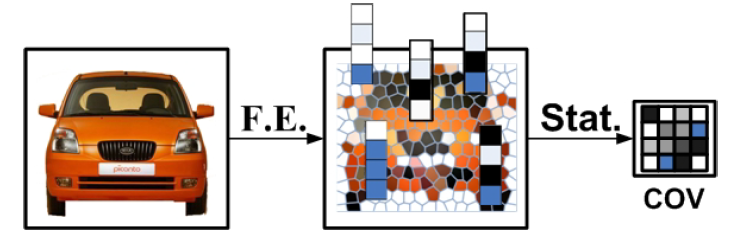
\includegraphics[width=0.7\linewidth]{images/sigmaset-fig1}
\caption{an image using $4\times 4$ covariance. "F.E."(feature extraction), "Stat" and "COV"}
\label{fig:sigmaset-fig1}
\end{figure}

For any matrix $A$ that satisfies $C_R=AA^T$, the set of columns of $A$ has the same 2nd order statistics as $R$. More specifically, we can construct the Sigma Set descriptor for region $R$ through Cholesky decomposition ($\mathbf{C} = \mathbf{L}\mathbf{L}^{\tiny{T}}$)  which is unique for SPD:
\begin{equation}
 S = \{\mathbf{L}_1, \cdots, \mathbf{L}_d, \mathbf{-L}_1, \cdots, \mathbf{-L}_d\}
\end{equation}
where $\mathbf{L}_i$ is th \textit{i}th column of $\sqrt{d}\times\mathbf{L}$.

An example application of sigma-set \cite{Uzair2013}.

\subsection{Kwatra2010}
"Fast Covariance Computation and
Dimensionality Reduction for Sub-Window Features in Images"

\subsubsection{Faulkner2015}
\cite{Faulkner2015} "A Study of the Region Covariance Descriptor: Impact of Feature Selection and Image Transformations"

%
% Super-pixels
%
\newpage
\section{Super-pixels}

\subsection{SLIC}
\cite{Achanta2012} this is a more efficient form of Superpixel. I have used this
in my previous work.

\subsection{Superpixel and salient objects}
\cite{He2015} "SuperCNN: A Superpixelwise Convolutional Neural Network for Salient Object Detection"

%
% Non-local Means
%
\newpage
\section{Non-Local Means}
\subsection{Qian2013}
\cite{Qian2013} 
nonlocal similarity and spectral-spatial structure of hyperspectral imagery into sparse representation. Non-locality means the self-similarity of image, by which a whole image can be partitioned into some groups containing similar patches. The similar patches in each group are sparsely represented with a shared subset of atoms in a dictionary making true signal and noise more easily separated.

\subsection{Fu2017}
\cite{Fu2017}

%
% K-means
%
\newpage
\section{K-means}

\subsection{Balanced K-means}
\cite{Malinen2014} 
in k-means assignment phase, the algorithm solves the assignment problem by Hungarian algorithm with time complexity $O(n^3)$.

\subsection{Balanced K-means \& min-cut}
\cite{Chang2014}


%
% SSD
%
\newpage
\section{SSD}

                                                                                             
%
% my research and implementation notes - not for publication
%
%\include{my_notes}

%\clearpage

\section{Conclusion}

\section{Remarks}


\vspace{24pt} \noindent\textbf{Acknowledgments.}{\small \quad
Finally, thank you to my family and friends for the support during this report.
}



\bibliographystyle{alpha}
\small{\bibliography{my-refs}}




%\appendix

\end{document}